\section{Estimation of Probability Upcrossing level $a$}
Connecting the Levy process with real-world case, one could take the change of stock price as an instance. The stock price probably fluctuates around the opening price instead of always surpassing or falling below. In our case, the linear drift of $\left\{X_{t}\right\}_{t \geq 0}$ given by $\mu T$ shall offset the effect of jumps in the long run. What is more concerning is that which coordinate of the discrete skeleton $\left\{\left(P_{i}, A_{i}, M_{i}\right)\right\}_{i \in \mathbb{N}}$ is more relevant to evaluate. The value of $M_i$ always records the highest level which $\left\{X_{t}\right\}_{t \geq 0}$ have ever reached before the $i^{th}$ jump. Then, for a path with $i$ jumps, if $M_i$ does not upcross level $a$, the path can never surpass level $a$.

\\
Figure \ref{fig:task5-3} shows 100 paths of simulated Lévy process. The mean of $Y_i$ for each path is set to be 1 and the drift factor $\mu$ to be -1. For the given value of $a$, the probability of $\left\{X_{t}\right\}_{t \geq 0}$ upcrossing level $a$ is calculated as the frequency of the exceeding paths over total simulated paths. Remind that, in this case, $\sigma$ is assigned to be 1 which leads to $\sigma B_t$ being a standard Brownian Motion. Thus, the probability of upcrossing is more likely to be determined by the variance of $(V_i-W_i)$ and $\sum_1^{N_t}Y_i$.
\begin{figure}[H]
    \centering
    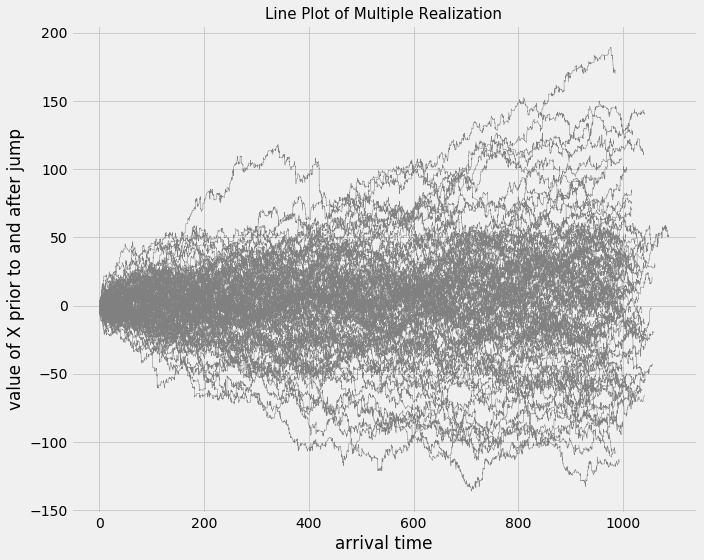
\includegraphics[scale = 0.45]{figures/task5-3.png}
    \caption{Simulation with $Y_i \sim {exp(\lambda = 1)}$, $\mu = -1$, $N_{jump} = 1000$, $\sigma$ = 1}
    \label{fig:task5-3}
\end{figure}

Figure \ref{fig:task5-4} illustrates the probability given different $a$-value. Considering $Y_i$ following the  exponential distribution, when the value of $a$ increases, the probability of $\left\{X_{t}\right\}_{t \geq 0}$ surpassing the given value decreases from 100\% to 0\%. If the level $a$ is set to be above 200, it almost never reaches within 1000 jumps. Meanwhile, considering all four different distributions of $Y_i$, the probability of upcrossing level $a$ conforms to the result of figure \ref{fig:task4} which mainly related to the variance of each distribution.

\begin{figure}[H]
    \centering
    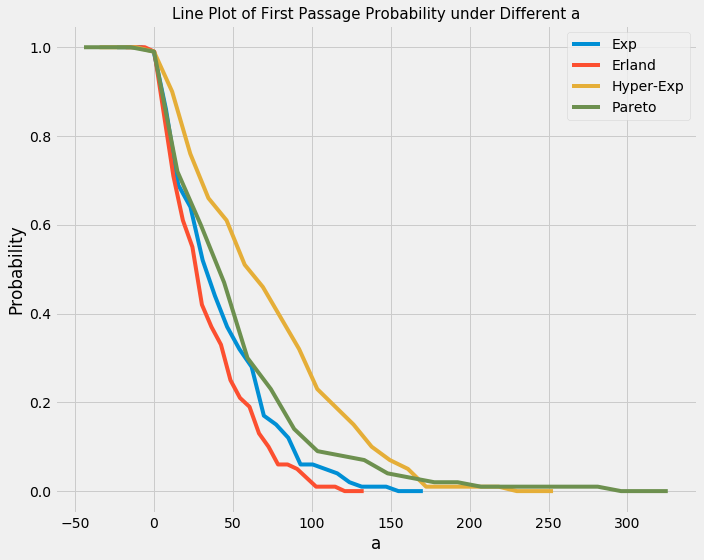
\includegraphics[scale = 0.45]{figures/task5-4.png}
    \caption{Fist passage probability of different distribution functions under different $a$ values}
    \label{fig:task5-4}
\end{figure}


\newpage




